\documentclass[11pt,a4paper]{report}%especifica o tipo de documento que tenciona escrever: carta, artigo, relatório... neste caso é um relatório
% [11pt,a4paper] Define o tamanho principal das letras do documento. caso não especifique uma delas, é assumido 10pt
% a4paper -- Define o tamanho do papel.

\usepackage[portuges]{babel}%Babel -- irá activar automaticamente as regras apropriadas de hifenização para a língua todo o
                                   %-- o texto gerado é automaticamente traduzido para Português.
                                   %  Por exemplo, “chapter” irá passar a “capítulo”, “table of contents” a “conteúdo”.
                                   % portuges -- específica para o Português.
\usepackage[utf8]{inputenc} % define o encoding usado texto fonte (input)--usual "utf8" ou "latin1

\usepackage{graphicx} %permite incluir graficos, tabelas, figuras
\usepackage{url} % para utilizar o comando \url{}
\usepackage{enumerate} %permite escolher, nas listas enumeradas, se os iems sao marcados com letras ou numeros-romanos em vez de numeracao normal

%\usepackage{apalike} % gerar biliografia no estilo 'named' (apalike)

\usepackage{color} % Para escrever em cores

\usepackage{multirow} %tabelas com multilinhas
\usepackage{array} %formatação especial de tabelas em array

\usepackage[pdftex]{hyperref} % transformar as referências internas do seu documento em hiper-ligações.

%Exemplos de fontes -- nao e vulgar mudar o tipo de fonte
%\usepackage{tgbonum} % Fonte de letra: TEX Gyre Bonum
%\usepackage{lmodern} % Fonte de letra: Latin Modern Sans Serif
%\usepackage{helvet}  % Fonte de letra: Helvetica
%\usepackage{charter} % Fonte de letra:Charter

\definecolor{saddlebrown}{rgb}{0.55, 0.27, 0.07} % para definir uma nova cor, neste caso 'saddlebrown'

\usepackage{listings}  % para utilizar blocos de texto verbatim no estilo 'listings'
%paramerização mais vulgar dos blocos LISTING - GENERAL
\lstset{
	basicstyle=\small, %o tamanho das fontes que são usadas para o código
	numbers=left, % onde colocar a numeração da linha
	numberstyle=\tiny, %o tamanho das fontes que são usadas para a numeração da linha
	numbersep=5pt, %distancia entre a numeração da linha e o codigo
	breaklines=true, %define quebra automática de linha
    frame=tB,  % caixa a volta do codigo
	mathescape=true, %habilita o modo matemático
	escapeinside={(*@}{@*)} % se escrever isto  aceita tudo o que esta dentro das marcas e nao altera
}
%
%\lstset{ %
%	language=Java,							% choose the language of the code
%	basicstyle=\ttfamily\footnotesize,		% the size of the fonts that are used for the code
%	keywordstyle=\bfseries,					% set the keyword style
%	%numbers=left,							% where to put the line-numbers
%	numberstyle=\scriptsize,				% the size of the fonts that are used for the line-numbers
%	stepnumber=2,							% the step between two line-numbers. If it's 1 each line
%											% will be numbered
%	numbersep=5pt,							% how far the line-numbers are from the code
%	backgroundcolor=\color{white},			% choose the background color. You must add \usepackage{color}
%	showspaces=false,						% show spaces adding particular underscores
%	showstringspaces=false,					% underline spaces within strings
%	showtabs=false,							% show tabs within strings adding particular underscores
%	frame=none,								% adds a frame around the code
%	%abovecaptionskip=-.8em,
%	%belowcaptionskip=.7em,
%	tabsize=2,								% sets default tabsize to 2 spaces
%	captionpos=b,							% sets the caption-position to bottom
%	breaklines=true,						% sets automatic line breaking
%	breakatwhitespace=false,				% sets if automatic breaks should only happen at whitespace
%	title=\lstname,							% show the filename of files included with \lstinputlisting;
%											% also try caption instead of title
%	escapeinside={\%*}{*)},					% if you want to add a comment within your code
%	morekeywords={*,...}					% if you want to add more keywords to the set
%}

\usepackage{xspace} % deteta se a seguir a palavra tem uma palavra ou um sinal de pontuaçao se tiver uma palavra da espaço, se for um sinal de pontuaçao nao da espaço

\parindent=0pt %espaço a deixar para fazer a  indentação da primeira linha após um parágrafo
\parskip=2pt % espaço entre o parágrafo e o texto anterior

\setlength{\oddsidemargin}{-1cm} %espaço entre o texto e a margem
\setlength{\textwidth}{18cm} %Comprimento do texto na pagina
\setlength{\headsep}{-1cm} %espaço entre o texto e o cabeçalho
\setlength{\textheight}{23cm} %altura do texto na pagina

% comando '\def' usado para definir abreviatura (macros)
% o primeiro argumento é o nome do novo comando e o segundo entre chavetas é o texto original, ou sequência de controle, para que expande
\def\darius{\textsf{Darius}\xspace}
\def\antlr{\texttt{AnTLR}\xspace}
\def\pe{\emph{Publicação Eletrónica}\xspace}
\def\titulo#1{\section{#1}}    %no corpo do documento usa-se na forma '\titulo{MEU TITULO}'
\def\super#1{{\em Supervisor: #1}\\ }
\def\area#1{{\em \'{A}rea: #1}\\[0.2cm]}
\def\resumo{\underline{Resumo}:\\ }

%\input{LPgeneralDefintions} %permite ler de um ficheiro de texto externo mais definições

\title{Processamento de Linguagens e Compiladores (3º ano de Curso)\\
       \textbf{Trabalho Prático nº 1
}\\ Relatório de Desenvolvimento\\-----------
\\Grupo nr. 10

       } %Titulo do documento
%\title{Um Exemplo de Artigo em \LaTeX}
\author{Bruno Neiva\\ (a95311) \and José Ferreira\\ (a96796) \and Moisés Ferreira\\ (a97020)
       } %autores do documento
\date{\today} %data

\begin{document} % corpo do documento
\maketitle % apresentar titulo, autor e data

\begin{abstract}  % resumo do documento
\\Neste trabalho prático, resolvemos os exercícios 1 e 2 do respetivo enunciado. O objetivo deste projeto é desenvolver a capacidade de utilizar \textit{Expressões Regulares (Er)} para filtrar/transformar textos com base no conceito de regras de produção \textit{Condição-Ação}.\\\
\end{abstract}

\tableofcontents % Insere a tabela de indice
%\listoffigures % Insere a tabela de indice figuras
%\listoftables % Insere a tabela de indice tabelas

\newpage
\chapter{ Processador de Registos de Exames Médicos Desportivos} \label{chap:ex2} %capitulo e referencia cruzada


\section{Análise do Problema 2} \label{sec:analiseProb2}
Neste problema recebemos um "dataset" gerado no âmbito do registo de exames médicos desportivos.
O objetivo deste problema era:

\begin{itemize}
  \item Calcular as idades extremas;
  \item Calcular a distribuição por Género no Total;
  \item Calcular a distribuição de Modalidades por ano;
  \item Calcular a distribuição de Modalidades no total;
  \item Calcular a percentagem de aptos e não aptos.
\end{itemize}

\newpage
\section{Resolução do Problema 2} \label{sec:resProb2}

Para a resolução deste problema recorremos às seguintes soluções sequenciadas:

\begin{enumerate}[i)]
     \item Criar um dicionário e alocar cada parâmetro do ficheiro csv;
     \item Calcular cada alínea individualmente; 
     \item Gerar uma página HTML para cada alínea com o seu resultado;
	 \item Gerar uma página HTML com todas os dados compilados.
  \end{enumerate}
  
  
  
\subsection{Criação e Alocação no Dicionário} \label{subsec:parser2}
Esta parte do problema foi resolvido com a função chamada filtrar\textunderscore csv\\
Esta função recebe o descritor de ficheiro do ficheiro emd.csv e separar por "new lines" de forma a obter as linhas da tabela. De seguida acede a cada coluna do ficheiro, separando por "," e usa Expressões Regulares para procurar os padrões de cada parâmetro e de seguida guardá-los num dicionário.

\begin{figure}[htbp]
\centerline{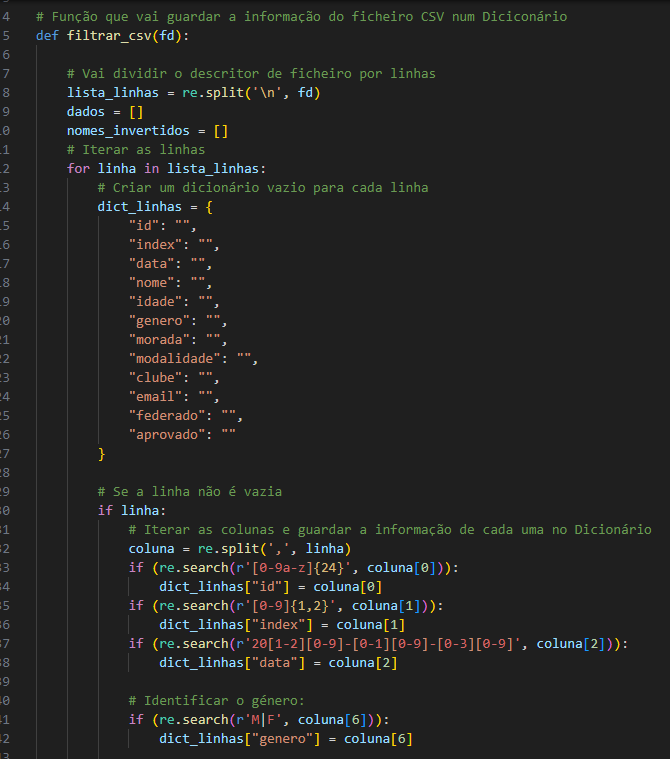
\includegraphics{filtrar_csv1.png}}
\caption{Excerto da função filtrar\textunderscore csv(fd) PARTE 1}
\label{fig}
\end{figure}  


Como se pode ver na figura anterior, cada entrada do ficheiro está agora seperada através da função split e estão guardados numa variável "lista\textunderscore linhas". Foi criado um dicionário onde foi guardada a informação de cada parâmetro através de outro split, onde em cada linha, foi obtida a informação de cada "coluna".\\

Conjuntos de Expressões Regulares utilizadas:

\begin{itemize}
  \item ER Id: \texttt{[0-9a-z]{24}};
  \item ER Index: \texttt{"[0-9]{1,2}"};
  \item ER Data: \texttt{"20[1-2][0-9]-[0-1][0-9]-[0-3][0-9]"};
  \item ER Nome: \texttt{"[A-Z][a-z]+"};
  \item ER Idade: \texttt{"[1-3][0-9]"};
  \item ER Género: \texttt{"M|F"};
  \item ER Morada: \texttt{"[A-Z][a-z]+"}
  \item ER Modalidade: \texttt{"[A-Za-zÀ-ÿ]+"}
  \item ER Clube: \texttt{"[A-Za-z]+"}
  \item ER Email: \texttt{"[a-z.]+[a-z]+@[a-z.]+"};
  \item ER Federado: \texttt{"true|false"};
  \item ER Apto: \texttt{"true|false"};
\end{itemize}


\begin{figure}[htbp]
\centerline{\includegraphics{filtra_info2_EX2.png}}
\caption{Excerto da função filtrar\textunderscore csv(fd) PARTE 2}
\label{fig}
\end{figure} 



\subsection{Cálculo das Alíneas} \label{subsec:indicadoresCalc}
Esta parte do problema foi resolvido com 5 funções distintas: extremos\textunderscore idade, genero\textunderscore total, modalidade\textunderscore ano, modalidade\textunderscore total, percentagem\textunderscore aptos.\\

\title{\textbf{extremos\textunderscore idade(dados)}}

Nesta função, percorremos o array de dicionários \textit{"dados"} onde foram guardadas as informações do ficheiro. Foram feitas sucessivas comparações do parâmetro idade e é retornado uma lista com a menor e maior idade.


\begin{figure}[htbp]
\centerline{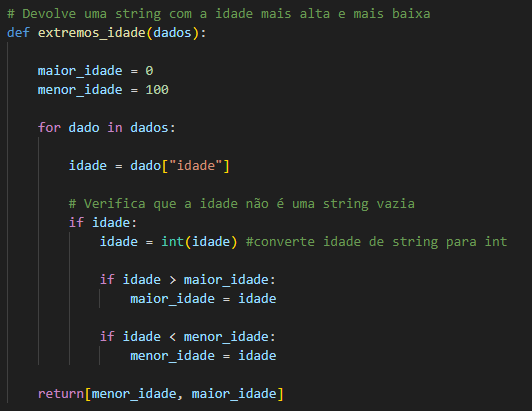
\includegraphics{extremos_idade.png}}
\caption{Função extremos\textunderscore idade(dados)}
\label{fig}
\end{figure}  

\newpage
\title{\textbf{genero\textunderscore total(dados)}}

Nesta função, iteramos o array e guardamos num dicionário o número total de pessoas do género Masculino e Feminino.\\

\begin{figure}[htbp]
\centerline{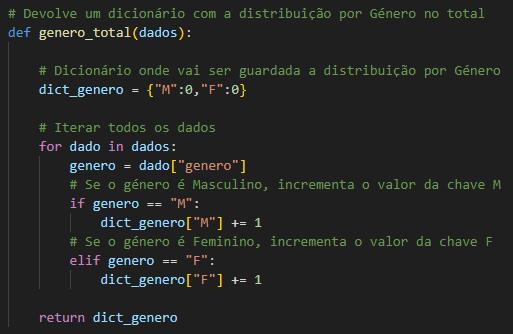
\includegraphics{genero_total.png}}
\caption{Função genero\textunderscore total(dados))}
\label{fig}
\end{figure}  

\title{\textbf{modalidade\textunderscore ano(dados)}}

Nesta função, iteramos o array e guardamos o ano numa variável para posteriormente usar como chave num dicionário. Nesse dicionário, criamos outro dicionário em que a modalidade era a chave e um contador era o valor.
\begin{figure}[htbp]
\centerline{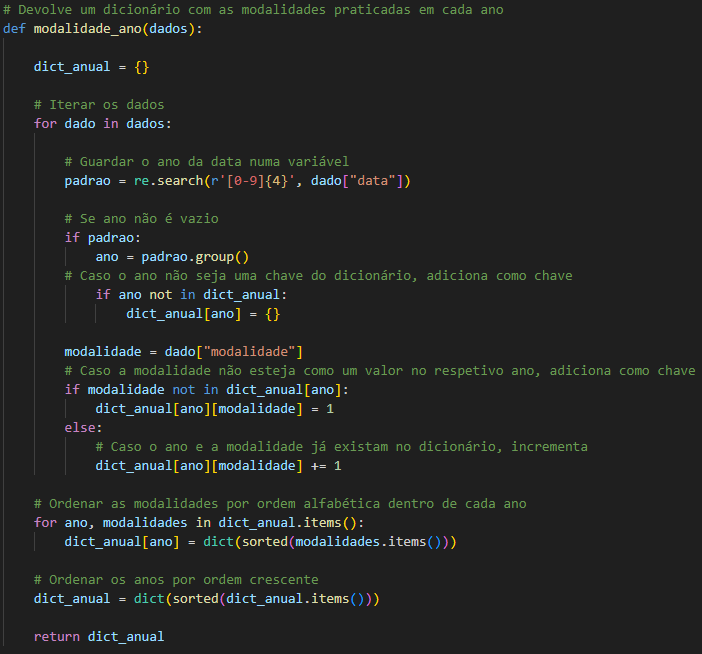
\includegraphics{modalidade_ano.png}}
\caption{Função modalidade\textunderscore ano(dados)}
\label{fig}
\end{figure}  

\newpage
\title{\textbf{modalidade\textunderscore total(dados)}}

Nesta função, iteramos o array e criamos um dicionário onde as modalidades eram a chave e o valor era um contador.\\
\begin{figure}[htbp]
\centerline{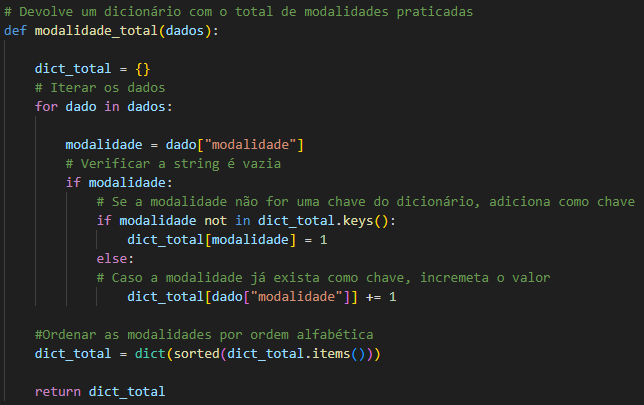
\includegraphics{modalidade_total.png}}
\caption{Função modalidade\textunderscore total(dados)}
\label{fig}
\end{figure} 

\title{\textbf{percentagem\textunderscore aptos(dados)}}

Nesta função, foi criado um dicionário onde foi guardado como chave true e false e um contador para cada uma dessas chaves. Foi calculado o total de pessoas ao somar o contador das duas chaves e de seguida foi calculado a percentagem de aptos e não aptos.
\begin{figure}[htbp]
\centerline{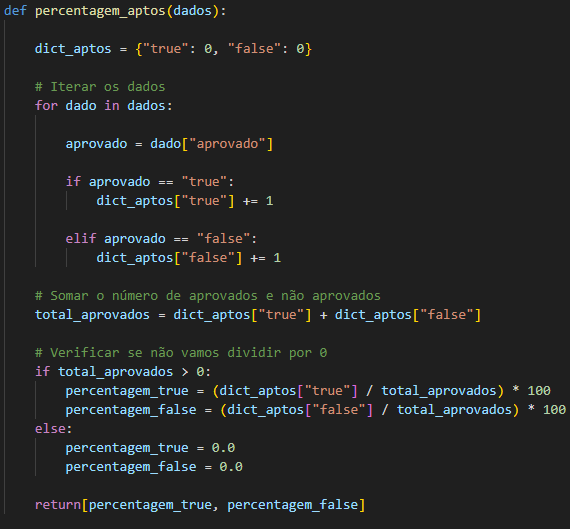
\includegraphics{percentagem_aptos.png}}
\caption{Função percentagem\textunderscore aptos(dados)}
\label{fig}
\end{figure}  



\newpage
\subsection{Páginas HTML de cada alínea} \label{subsec:indicadoresTable}
Esta parte do problema foi resolvido com 5 funções distintas: gerar\textunderscore html\textunderscore extremos\textunderscore idade(idades), gerar\textunderscore html\textunderscore genero\textunderscore total(dict\textunderscore generos), gerar\textunderscore html\textunderscore modalidade\textunderscore ano(dados\textunderscore modalidade), gerar\textunderscore html\textunderscore modalidades\textunderscore total(dados\textunderscore modalidades), gerar\textunderscore html\textunderscore percentagem\textunderscore aptos(dados\textunderscore aptos)\\

\title{\textbf{gerar\textunderscore html\textunderscore extremos\textunderscore idade(idades)}}

Esta função é responsável por gerar o código html da página idades.html onde é escrito o resultado da função extremos\textunderscore idade.


\begin{figure}[htbp]
\centerline{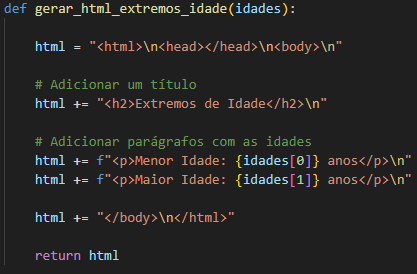
\includegraphics{gerar_html_extremos_idade.png}}
\caption{Função gerar\textunderscore html\textunderscore extremos\textunderscore idade(idades)}
\label{fig}
\end{figure}  

\newpage
\title{\textbf{gerar\textunderscore html\textunderscore genero\textunderscore total(generos)}}

Esta função é responsável por gerar o código html da página generos.html onde é escrito o resultado da função genero\textunderscore total.


\begin{figure}[htbp]
\centerline{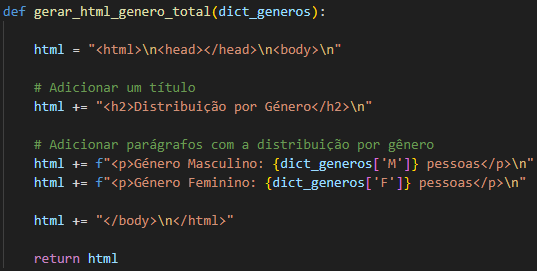
\includegraphics[scale=0.8]{gerar_html_genero_total.png}}
\caption{Função gerar\textunderscore html\textunderscore genero\textunderscore total(generos)}
\label{fig}
\end{figure}  


\title{\textbf{gerar\textunderscore html\textunderscore modalidade\textunderscore ano(dados\textunderscore modalidade)}}

Esta função é responsável por gerar o código html da página modalidades\textunderscore anual.html onde é escrito o resultado da função modalidade\textunderscore ano.


\begin{figure}[htbp]
\centerline{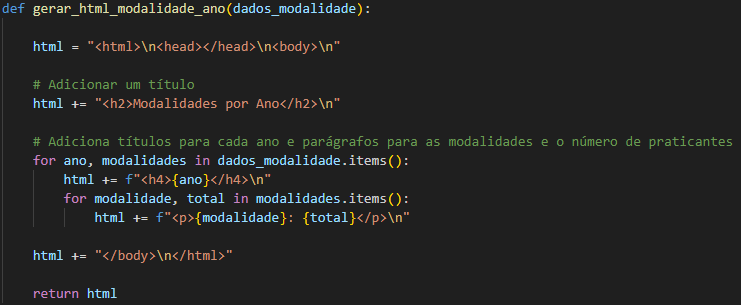
\includegraphics[scale=0.8]{gerar_html_modalidade_ano.png}}
\caption{Função gerar\textunderscore html\textunderscore modalidade\textunderscore ano(dados\textunderscore modalidade)}
\label{fig}
\end{figure}


\newpage
\title{\textbf{gerar\textunderscore html\textunderscore modalidades\textunderscore total(dados\textunderscore modalidades)}}

Esta função é responsável por gerar o código html da página modalidades\textunderscore total.html onde é escrito o resultado da função modalidade\textunderscore total.


\begin{figure}[htbp]
\centerline{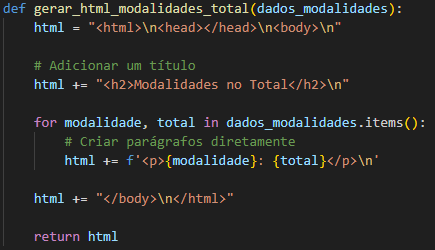
\includegraphics[scale=0.8]{gerar_html_modalidades_total.png}}
\caption{Função gerar\textunderscore html\textunderscore modalidades\textunderscore total(dados\textunderscore modalidades)}
\label{fig}
\end{figure}


\newpage
\title{\textbf{gerar\textunderscore html\textunderscore percentagem\textunderscore aptos(dados\textunderscore aptos)}}

Esta função é responsável por gerar o código html da página aptos.html onde é escrito o resultado da função percentagem\textunderscore aptos.


\begin{figure}[htbp]
\centerline{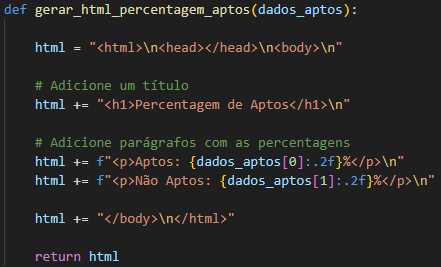
\includegraphics[scale=0.8]{gerar_html_percentagem_aptos.png}}
\caption{Função gerar\textunderscore html\textunderscore percentagem\textunderscore aptos(dados\textunderscore aptos)}
\label{fig}
\end{figure} 



\newpage
\subsection{Gerar página HTML final} \label{subsec:htmlGenerator}
Nesta parte, criamos uma página index.html onde foi compilada a informação de cada página html gerada em cada alínea.


\begin{figure}[htbp]
\centerline{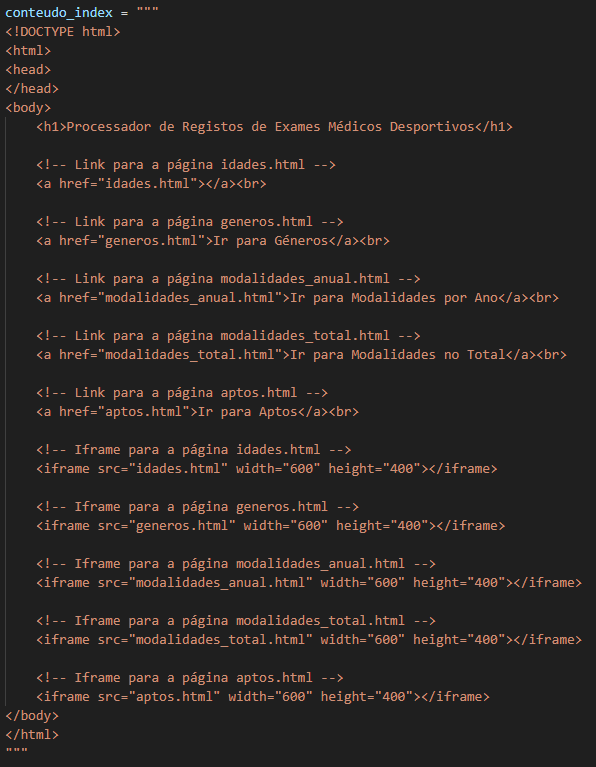
\includegraphics{gerar_index_html.png}}
\caption{Código usado para gerar a página index.html}
\label{fig}
\end{figure}


\newpage
\section{Resultados do Problema 2} \label{sec:resProb2} %seccao e referencia cruzada
\subsection{Página index.html} \label{subsec:indc}
Aqui temos o conteúdo do ficheiro "index.html".

\begin{figure}[htbp]
\centerline{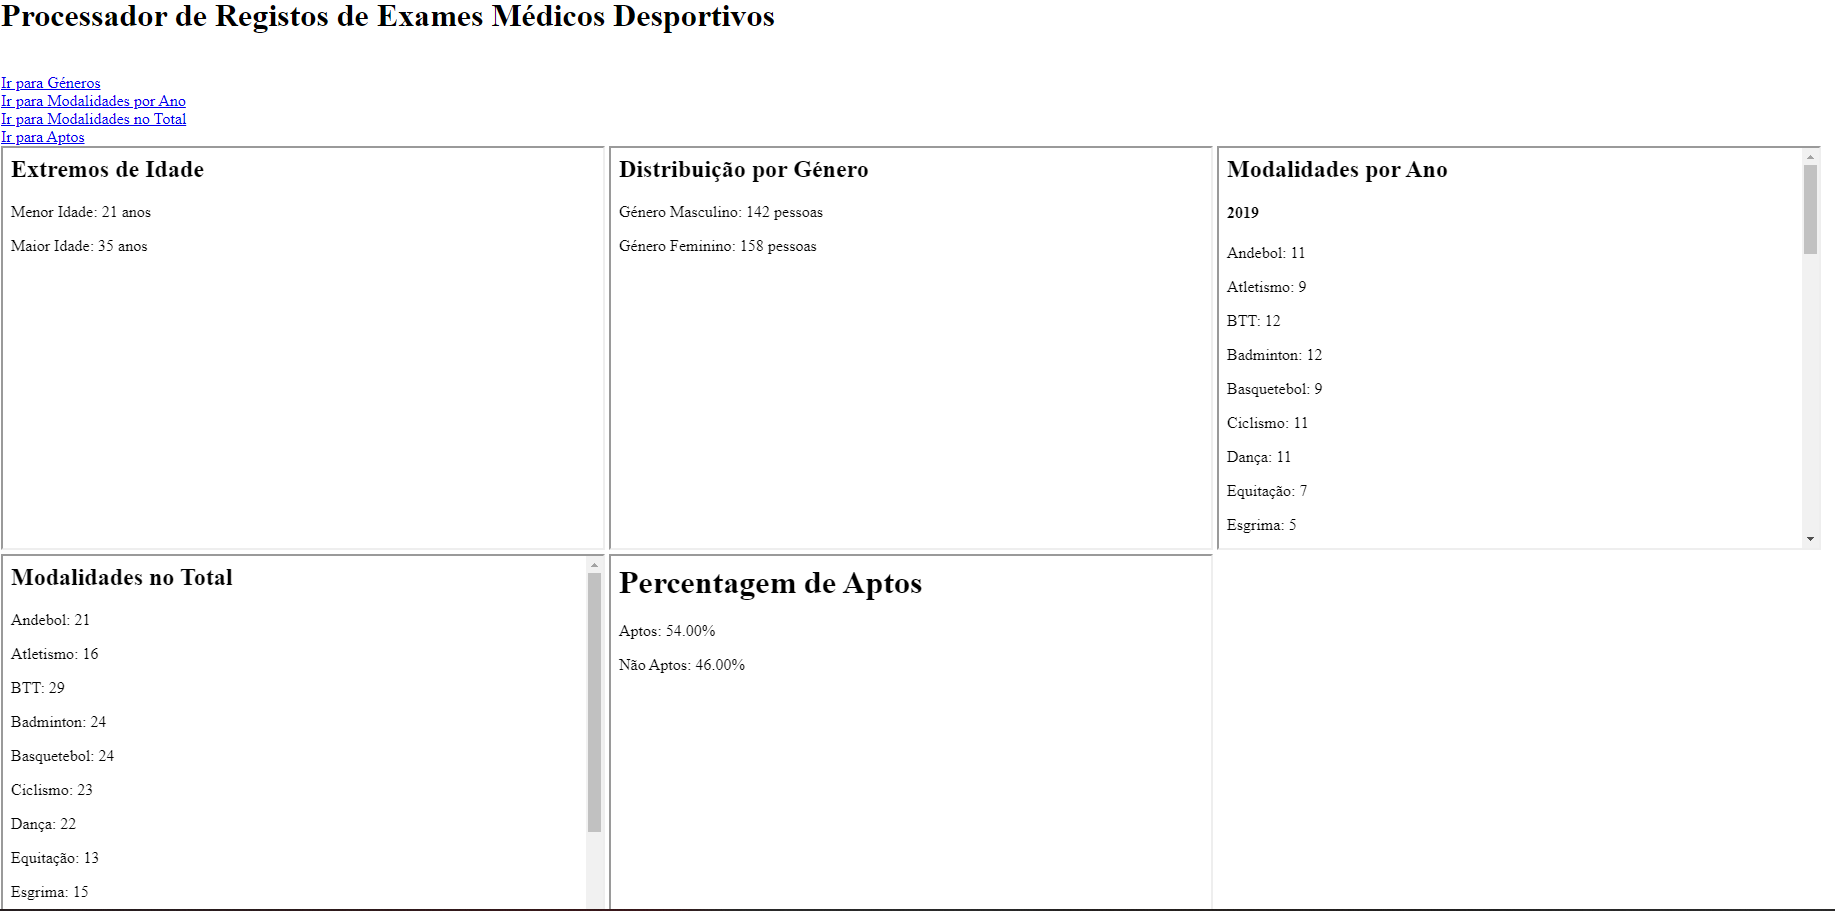
\includegraphics[scale=0.7]{index_html.png}}
\caption{Conteúdo do ficheiro index.html}
\label{fig}
\end{figure}

\chapter{Conclusão} \label{concl}
A realização deste trabalho prático possibilitou a consolidação da matéria lecionada sobre Expressões Regulares e também desenvolver mais conhecimentos sobre Python e HTML.\\
Em especifico este projeto permitiu-nos aprimorar a escrita de ER para resolução de problemas e filtragem de texto, bem como a a utilização do módulo 're' e as suas funções.\\
\appendix % apendice
\chapter{Código do Programa}
\begin{verbatim}
import re
import json

# Função que vai guardar a informação do ficheiro CSV num Diciconário               
def filtrar_csv(fd):

    # Vai dividir o descritor de ficheiro por linhas
    lista_linhas = re.split('\n', fd)
    dados = []
    nomes_invertidos = []
    # Iterar as linhas
    for linha in lista_linhas:
        # Criar um dicionário vazio para cada linha
        dict_linhas = {
            "id": "",
            "index": "",
            "data": "",
            "nome": "",
            "idade": "",
            "genero": "",
            "morada": "",
            "modalidade": "",
            "clube": "",
            "email": "",
            "federado": "",
            "aprovado": ""
        }

        # Se a linha não é vazia
        if linha:
            # Iterar as colunas e guardar a informação de cada uma no Dicionário
            coluna = re.split(',', linha)
            if (re.search(r'[0-9a-z]{24}', coluna[0])):
                dict_linhas["id"] = coluna[0]
            if (re.search(r'[0-9]{1,2}', coluna[1])):
                dict_linhas["index"] = coluna[1]
            if (re.search(r'20[1-2][0-9]-[0-1][0-9]-[0-3][0-9]', coluna[2])):
                dict_linhas["data"] = coluna[2]

            # Identificar o género:
            if (re.search(r'M|F', coluna[6])):
                dict_linhas["genero"] = coluna[6]

            # Normalizar os nomes:    
            if (re.search(r'[A-Z][a-z]+', coluna[3])):
                # Se o género for Feminino, escreve o nome pela ordem do documento
                if dict_linhas["genero"] == 'F' and re.search(r'[A-Z][a-z]+', coluna[4]):
                    dict_linhas["nome"] = coluna[3] + " " + coluna[4]

                else:
                # Caso seja Masculino, inverte a ordem e guarda os nomes trocados num array
                    if (re.search(r'[A-Z][a-z]+', coluna[4])):
                        dict_linhas["nome"] = coluna[4] + " " + coluna[3]
                        nomes_invertidos.append({
                            "Nome Original": coluna[3] + " " + coluna[4],
                            "Nome Invertido": coluna[4] + " " + coluna[3]
                        })

            if (re.search(r'[1-3][0-9]', coluna[5])):
                dict_linhas["idade"] = coluna[5]
            
            if (re.search(r'[A-Z][a-z]+', coluna[7])):
                dict_linhas["morada"] = coluna[7]
            if (re.search(r'[A-Za-zÀ-ÿ]+', coluna[8])):
                dict_linhas["modalidade"] = coluna[8]
            if (re.search(r'[A-Za-z]+', coluna[9])):
                dict_linhas["clube"] = coluna[9]
            if (re.search(r'[a-z.]+[a-z]+@[a-z.]+', coluna[10])):
                dict_linhas["email"] = coluna[10]
            if (re.search(r'true|false', coluna[11])):
                dict_linhas["federado"] = coluna[11]
            if (re.search(r'true|false', coluna[12])):
                dict_linhas["aprovado"] = coluna[12]

        # Se o id não estiver vazio, dá append para o array
        if (dict_linhas["id"] != ""):
            dados.append(dict_linhas)

    return dados, nomes_invertidos


# Devolve uma string com a idade mais alta e mais baixa
def extremos_idade(dados):

    maior_idade = 0
    menor_idade = 100

    for dado in dados:

        idade = dado["idade"]

        # Verifica que a idade não é uma string vazia
        if idade:
            idade = int(idade) #converte idade de string para int

            if idade > maior_idade:
                maior_idade = idade
            
            if idade < menor_idade:
                menor_idade = idade

    return[menor_idade, maior_idade]


# Devolve um dicionário com a distribuição por Género no total
def genero_total(dados):

    # Dicionário onde vai ser guardada a distribuição por Género
    dict_genero = {"M":0,"F":0}

    # Iterar todos os dados 
    for dado in dados:
        genero = dado["genero"]
        # Se o género é Masculino, incrementa o valor da chave M
        if genero == "M":
            dict_genero["M"] += 1
        # Se o género é Feminino, incrementa o valor da chave F
        elif genero == "F":
            dict_genero["F"] += 1

    return dict_genero


# Devolve um dicionário com as modalidades praticadas em cada ano
def modalidade_ano(dados):

    dict_anual = {}

    # Iterar os dados
    for dado in dados:
        
        # Guardar o ano da data numa variável
        padrao = re.search(r'[0-9]{4}', dado["data"])

        # Se ano não é vazio
        if padrao:
            ano = padrao.group() 
        # Caso o ano não seja uma chave do dicionário, adiciona como chave
            if ano not in dict_anual:
                dict_anual[ano] = {}
        
        modalidade = dado["modalidade"]
        # Caso a modalidade não esteja como um valor no respetivo ano, adiciona como chave
        if modalidade not in dict_anual[ano]:
            dict_anual[ano][modalidade] = 1
        else:
            # Caso o ano e a modalidade já existam no dicionário, incrementa
            dict_anual[ano][modalidade] += 1

    # Ordenar as modalidades por ordem alfabética dentro de cada ano
    for ano, modalidades in dict_anual.items():
        dict_anual[ano] = dict(sorted(modalidades.items()))
    
    # Ordenar os anos por ordem crescente
    dict_anual = dict(sorted(dict_anual.items()))

    return dict_anual


# Devolve um dicionário com o total de modalidades praticadas
def modalidade_total(dados):

    dict_total = {}
    # Iterar os dados
    for dado in dados:

        modalidade = dado["modalidade"]
        # Verificar a string é vazia
        if modalidade:
            # Se a modalidade não for uma chave do dicionário, adiciona como chave
            if modalidade not in dict_total.keys():
                dict_total[modalidade] = 1
            else:
            # Caso a modalidade já exista como chave, incremeta o valor
                dict_total[dado["modalidade"]] += 1

    #Ordenar as modalidades por ordem alfabética
    dict_total = dict(sorted(dict_total.items()))

    return dict_total


def percentagem_aptos(dados):

    dict_aptos = {"true": 0, "false": 0}

    # Iterar os dados
    for dado in dados:

        aprovado = dado["aprovado"]

        if aprovado == "true":
            dict_aptos["true"] += 1

        elif aprovado == "false":
            dict_aptos["false"] += 1
    
    # Somar o número de aprovados e não aprovados
    total_aprovados = dict_aptos["true"] + dict_aptos["false"]

    # Verificar se não vamos dividir por 0
    if total_aprovados > 0:
        percentagem_true = (dict_aptos["true"] / total_aprovados) * 100
        percentagem_false = (dict_aptos["false"] / total_aprovados) * 100
    else:
        percentagem_true = 0.0
        percentagem_false = 0.0

    return[percentagem_true, percentagem_false]


# Abrir o ficheiro emd.csv e executar a função filtrar_csv
ficheiro_filtrado = []
with open("emd.csv") as file:
    fd = file.read()
    ficheiro_filtrado, nomes_invertidos = filtrar_csv(fd)


# Guardar os nomes trocados num ficheiro em formato JSON
with open("nomes_invertidos.json", "w") as json_file:
    json.dump(nomes_invertidos, json_file, indent=4)


# ---------------------------------------------------------------------
# GERAR AS PÁGINAS HTML ONDE SERÃO IMPRIMIDOS OS RESULTADOS DAS FUNÇÕES
# ---------------------------------------------------------------------

idades = extremos_idade(ficheiro_filtrado) 

def gerar_html_extremos_idade(idades):  

    html = "<html>\n<head></head>\n<body>\n"
    
    # Adicionar um título
    html += "<h2>Extremos de Idade</h2>\n"

    # Adicionar parágrafos com as idades
    html += f"<p>Menor Idade: {idades[0]} anos</p>\n"
    html += f"<p>Maior Idade: {idades[1]} anos</p>\n"
    
    html += "</body>\n</html>"

    return html

html_extremos_idade = gerar_html_extremos_idade(idades)

# Escrever a string HTML no ficheiro idades.html
with open("idades.html", "w") as file:
    file.write(html_extremos_idade)



generos = genero_total(ficheiro_filtrado)

def gerar_html_genero_total(dict_generos):

    html = "<html>\n<head></head>\n<body>\n"
    
    # Adicionar um título
    html += "<h2>Distribuição por Género</h2>\n"

    # Adicionar parágrafos com a distribuição por gênero
    html += f"<p>Género Masculino: {dict_generos['M']} pessoas</p>\n"
    html += f"<p>Género Feminino: {dict_generos['F']} pessoas</p>\n"
    
    html += "</body>\n</html>"

    return html

html_genero_total = gerar_html_genero_total(generos)

# Escrever a string HTML no ficheiro generos.html
with open("generos.html", "w") as file:
    file.write(html_genero_total)



dados_modalidades_anual = modalidade_ano(ficheiro_filtrado)

def gerar_html_modalidade_ano(dados_modalidade):

    html = "<html>\n<head></head>\n<body>\n"

    # Adicionar um título
    html += "<h2>Modalidades por Ano</h2>\n"

    # Adiciona títulos para cada ano e parágrafos para as modalidades e o número de praticantes
    for ano, modalidades in dados_modalidade.items():
        html += f"<h4>{ano}</h4>\n"
        for modalidade, total in modalidades.items():
            html += f"<p>{modalidade}: {total}</p>\n"

    html += "</body>\n</html>"

    return html

html_modalidade_ano = gerar_html_modalidade_ano(dados_modalidades_anual)

# Escrever a string HTML no ficheiro modalidades_anual.html
with open("modalidades_anual.html", "w") as file:
    file.write(html_modalidade_ano)



dados_modalidades_total = modalidade_total(ficheiro_filtrado)

def gerar_html_modalidades_total(dados_modalidades):
    html = "<html>\n<head></head>\n<body>\n"

    # Adicionar um título
    html += "<h2>Modalidades no Total</h2>\n"
    
    for modalidade, total in dados_modalidades.items():
        # Criar parágrafos diretamente
        html += f'<p>{modalidade}: {total}</p>\n'
    
    html += "</body>\n</html>"

    return html

html_modalidades_total = gerar_html_modalidades_total(dados_modalidades_total)

# Escrever a string HTML no ficheiro modalidades_total.html
with open("modalidades_total.html", "w") as file:
    file.write(html_modalidades_total)



aptos = percentagem_aptos(ficheiro_filtrado)

def gerar_html_percentagem_aptos(dados_aptos):

    html = "<html>\n<head></head>\n<body>\n"
    
    # Adicione um título
    html += "<h1>Percentagem de Aptos</h1>\n"

    # Adicione parágrafos com as percentagens
    html += f"<p>Aptos: {dados_aptos[0]:.2f}%</p>\n"
    html += f"<p>Não Aptos: {dados_aptos[1]:.2f}%</p>\n"
    
    html += "</body>\n</html>"

    return html


html_percentagem_aptos = gerar_html_percentagem_aptos(aptos)

# Escrever a string HTML no arquivo aptos.html
with open("aptos.html", "w") as file:
    file.write(html_percentagem_aptos)


conteudo_index = """
<!DOCTYPE html>
<html>
<head>
</head>
<body>
    <h1>Processador de Registos de Exames Médicos Desportivos</h1>
    
    <!-- Link para a página idades.html -->
    <a href="idades.html"></a><br>

    <!-- Link para a página generos.html -->
    <a href="generos.html">Ir para Géneros</a><br>

    <!-- Link para a página modalidades_anual.html -->
    <a href="modalidades_anual.html">Ir para Modalidades por Ano</a><br>

    <!-- Link para a página modalidades_total.html -->
    <a href="modalidades_total.html">Ir para Modalidades no Total</a><br>

    <!-- Link para a página aptos.html -->
    <a href="aptos.html">Ir para Aptos</a><br>

    <!-- Iframe para a página idades.html -->
    <iframe src="idades.html" width="600" height="400"></iframe>

    <!-- Iframe para a página generos.html -->
    <iframe src="generos.html" width="600" height="400"></iframe>

    <!-- Iframe para a página modalidades_anual.html -->
    <iframe src="modalidades_anual.html" width="600" height="400"></iframe>

    <!-- Iframe para a página modalidades_total.html -->
    <iframe src="modalidades_total.html" width="600" height="400"></iframe>

    <!-- Iframe para a página aptos.html -->
    <iframe src="aptos.html" width="600" height="400"></iframe>
</body>
</html>
"""

with open("index.html", "w") as file:
    file.write(conteudo_index)

\end{verbatim}

\end{document} 

